\sectionframe{Abbildung logischer Ausdrücke}
\begin{frame}
 \frametitle{Beispiel: Adventure Inc.}
 \begin{figure}
  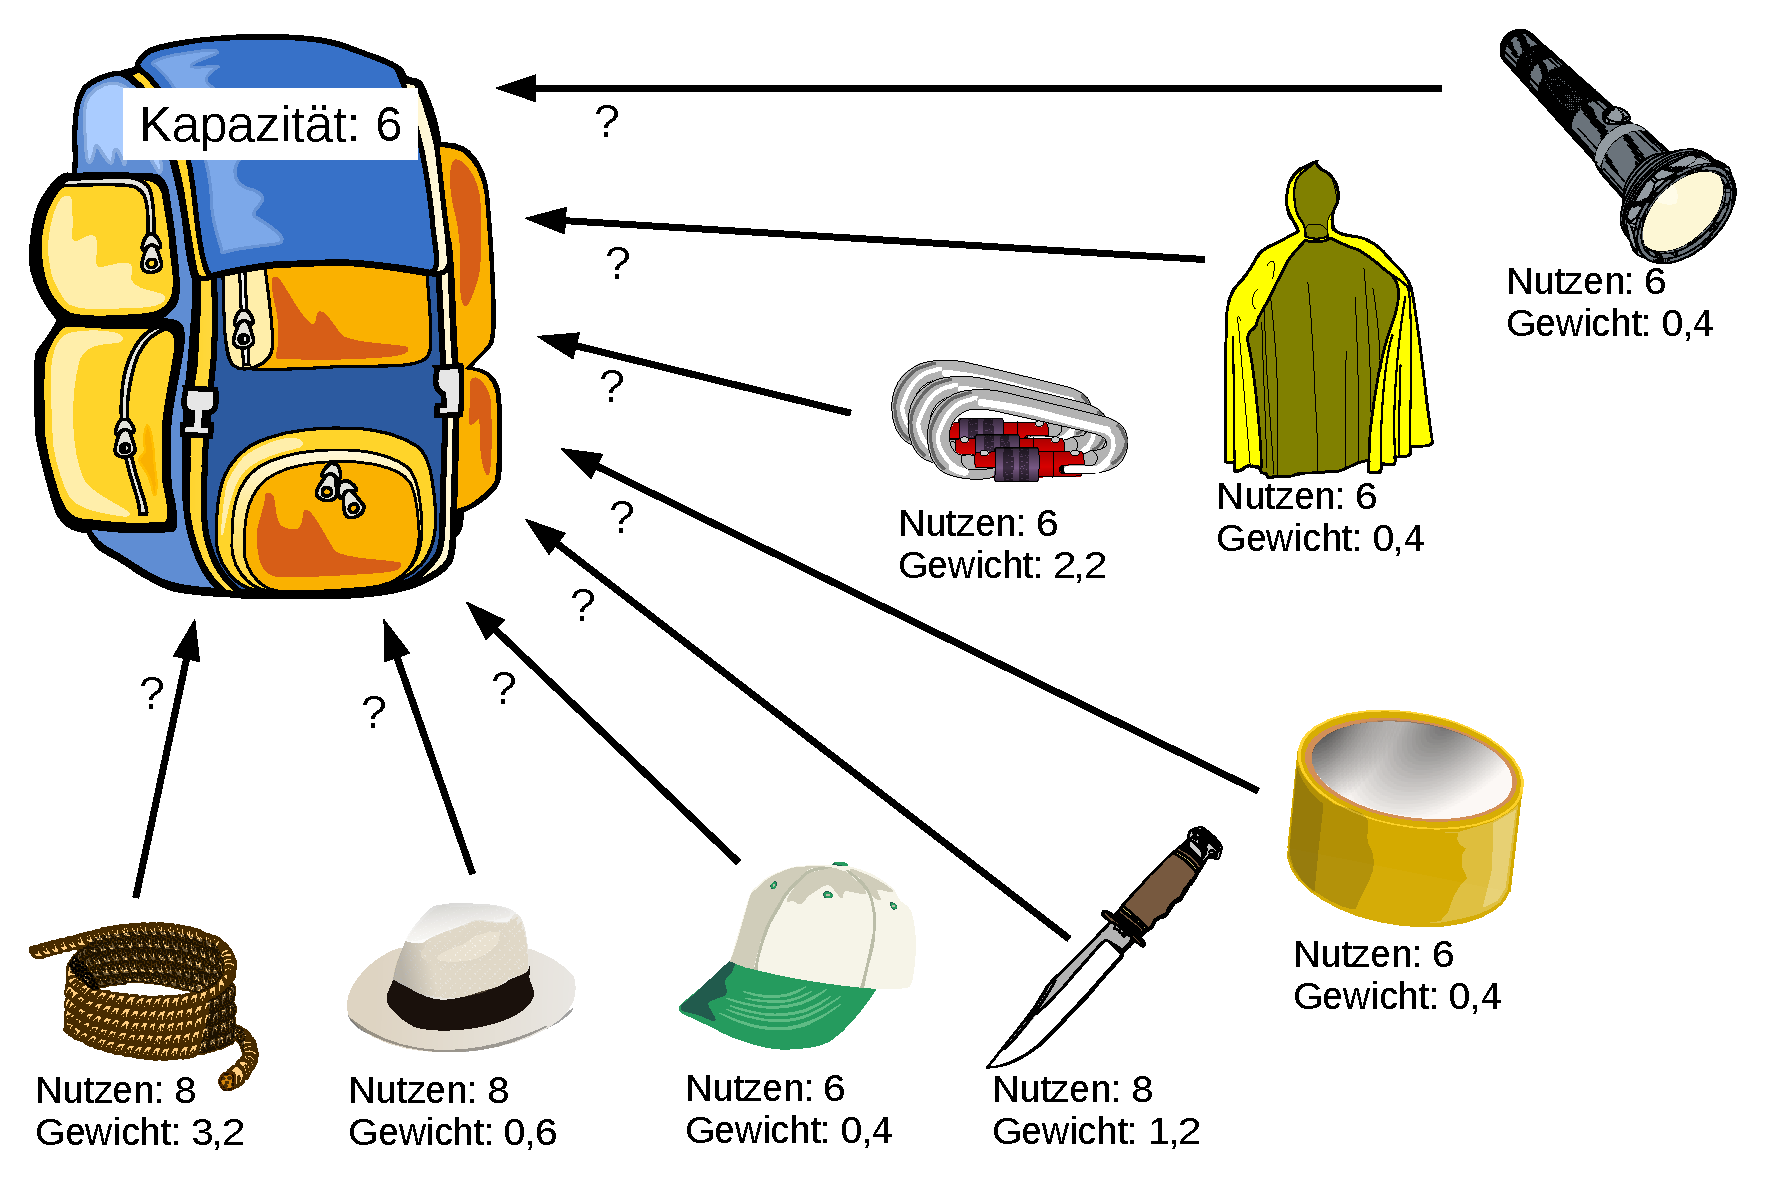
\includegraphics[width=\linewidth]{Bilder/Rucksackproblem}
 \end{figure}
\end{frame}

\begin{frame}\small
 \frametitle{Modell: Rucksackproblem}
 \begin{tabularx}{\linewidth}{lL}
  \multicolumn{2}{l}{\textbf{Indexmengen}:}\\
    $I$ & Menge der Gegenstände\\
  \multicolumn{2}{l}{\textbf{Parameter}:}\\
    $w_i$ & Gewicht von Gegenstand~$i\in I$\\
    $u_i$ & Nutzen von Gegenstand~$i\in I$\\
    $c$ & Kapazität des Rucksacks\\
  \multicolumn{2}{l}{\textbf{Entscheidungsvariablen}:}\\
    $x_i$ & Binäre Entscheidungsvariable; zeigt an ob Gegenstand~$i\in I$ eingepackt wird\\[1ex]
  \multicolumn{2}{l}{\textbf{Modellbeschreibung}:}\\[1ex]
  \multicolumn{2}{l}{
	$
	\begin{array}{rllr}
	  \max & \displaystyle\sum_{i\in I} u_i\cdot x_i & & \\[3ex]
	  s.t. & \displaystyle\sum_{i\in I} w_i\cdot x_i \leq c & & \mathrm{(I)}\\
		  & \alert{x_i \in \{0,1\}} & \quad\forall i\in I & \\
	\end{array}
	$ 
  }\\[1ex]
 \end{tabularx}
\end{frame}

\begin{frame}
 \frametitle{Logische Verknüpfungen}
 \begin{description}
 \item[$\neg$] Die logische \textbf{{Negation}}  
 \item[$\wedge$] Das logische \textbf{{Und}}
 \item[$\vee$] Das logische \textbf{{Oder}}
 \item[$\veebar$] Das logische \textbf{exklusive Oder}("`Entweder-Oder"')
 \item[$\Rightarrow$] Die logische \textbf{{Implikation}}
 \item[$\Leftrightarrow$] Die logische \textbf{{Äquivalenz}}
\end{description}
\begin{block}{Wahrheitstafel in numerischer Beschreibung}
 \centering\footnotesize
 \begin{tabular}{*{9}{c}}
  \toprule
  $A$ & $B$ & $\neg A$ & $\neg B$ & $A\wedge B$ & $A\vee B$ & $A \veebar B$ & $A\Rightarrow B$ & $A\Leftrightarrow B$\\
  \midrule
  1 & 1 & 0 & 0 & 1 & 1 & 0 & 1 & 1\\
  1 & 0 & 0 & 1 & 0 & 1 & 1 & 0 & 0\\
  0 & 1 & 1 & 0 & 0 & 1 & 1 & 1 & 0\\
  0 & 0 & 1 & 1 & 0 & 0 & 0 & 1 & 1\\
  \bottomrule
 \end{tabular}
\end{block}
\end{frame}

\begin{frame}
 \frametitle{Logische Verknüpfungen in binären Optimierungsmodellen}
 {\small Beispiel: Seien $x_1$ und $x_2$ binäre Entscheidungsvariablen eines Rucksackproblems, die angeben, ob die Gegenstände $I_1$ und $I_2$ eingepackt werden.}
 \begin{center}\footnotesize
\begin{description}
  \only<1>{\item[$\neg I_1$:] Man möchte wissen ob $I_1$ nicht eingepackt ist.
  \begin{itemize}\item$
    1-x_1
  $\end{itemize}}
  \only<1>{\item[$I_1\wedge I_2$:]  Sowohl Gegenstand $1$ als auch Gegenstand $2$ müssen eingepackt werden.
  \begin{itemize}\item$
    x_1+x_2 = 2
  $\end{itemize}}
  \only<1>{\item[$I_1\vee I_2$:]  Mindestens einer der Gegenstände muss eingepackt werden.
  \begin{itemize}\item$
    x_1+x_2 \geq 1
  $\end{itemize}}
  \only<1>{\item[$\neg(I_1\wedge I_2)$:]  Höchstens einer der Gegenstände darf eingepackt werden.
  \begin{itemize}\item$
    x_1+x_2 \leq 1
  $\end{itemize}}
  \only<2>{\item[$\neg(I_1\vee I_2)$:]  Keiner der Gegenstände darf eingepackt werden. 
  \begin{itemize}\item$
    x_1+x_2 = 0
  $\end{itemize}}
  \only<2>{\item[$I_1\veebar I_2$:]  Genau einer der Gegenstände muss eingepackt werden. 
  \begin{itemize}\item$
    x_1+x_2 = 1
  $\end{itemize}}
  \only<2>{\item[$I_1\Rightarrow I_2$:]  Wenn $I_1$ eingepackt ist, muss auch $I_2$ eingepackt werden. 
  \begin{itemize}\item$
    x_1 \leq x_2
  $\end{itemize}}
  \only<2>{\item[$I_1\Leftrightarrow I_2$:]  Die Entscheidung für beide Gegenstände ist identisch. 
  \begin{itemize}\item$
    x_1 = x_2
  $\end{itemize}}
\end{description}
 \end{center}
\end{frame}
